%% template for IEICE Transactions
%% v2.1 [2015/10/31]
\documentclass[paper]{ieice}
% \usepackage{hyperref}
\usepackage{booktabs}
\usepackage{graphicx}
%\usepackage{caption}
\usepackage{nicefrac}
%\usepackage{subcaption}
\usepackage[T1]{fontenc}

%\usepackage{lmodern}
\usepackage{xspace}
\usepackage{flushend}  
\usepackage{color}
\usepackage{url}
\usepackage{booktabs}
\usepackage[table,xcdraw]{xcolor}
%\usepackage{colorbox}
\usepackage{multirow}
\usepackage{listliketab}
\usepackage{amssymb}
\usepackage{algorithm}
\usepackage{algorithmic}
\usepackage{booktabs}
%\usepackage{ascmac}%
\usepackage{comment}
\usepackage{amsmath}
\usepackage{pgfplots}
%\usepackage{arydshln}%
%\usepackage{fancybox}
\usepackage{bbding}
\usepackage{listings}
\usepackage{float}
% \usepackage{subfig}
\usepackage{tabularx}
\usepackage{cite}
\usepackage{rotating}
\usepackage[table,xcdraw]{xcolor}
\usepackage[square,sort,comma,numbers]{natbib}
\usepackage{tcolorbox}
\usepackage{ulem}
\usepackage{censor}
\usepackage{tikz}
\usepackage{amssymb} 
\usepackage{amsfonts}
\usepackage{graphicx,subfigure}
%\usepackage{xfp}
\usepackage{xparse}
\usepackage[colorinlistoftodos]{todonotes}
\usepackage{ulem}
\usepackage{amssymb}
\usepackage{lmodern}
\usepackage{mathtools, nccmath}
\usepackage{venndiagram}
\newcommand\wang[1]{{\textcolor{red}{W:#1}}}
%\documentclass[invited]{ieice}
%\documentclass[position]{ieice}
%\documentclass[survey]{ieice}
%\documentclass[invitedsurvey]{ieice}
%\documentclass[review]{ieice}
%\documentclass[tutorial]{ieice}
%\documentclass[letter]{ieice}
%\documentclass[brief]{ieice}
%\usepackage[dvips]{graphicx}
%\usepackage[pdftex]{graphicx,xcolor}
% \usepackage[dvipdfmx]{graphicx,xcolor}
% \usepackage[fleqn]{amsmath}
% \usepackage{newtxtext}
% \usepackage[varg]{newtxmath}
\usepackage{balance}
\usepackage{esvect}
\usepackage[colorlinks = true,
            linkcolor = blue,
            urlcolor  = blue,
            citecolor = blue,
            anchorcolor = blue]{hyperref}

\setcitestyle{square}

\newcommand{\RQOne}{\textbf{RQ$_1$: How do SO library usage patterns differ from actual projects patterns?}}
\newcommand{\PSOne}{\textit{What library usage patterns can we infer from SO posts?}}
\newcommand{\PSTwo}{\textit{How do inferred library usage patterns from SO compare to actual usage patterns?}}

% \newcommand{\RqOne}{\textbf{RQ$_1$: How does SOLibRec compare with the state of art approach in term of success rate?}}

% \newcommand{\RqTwo}{\textbf{RQ$_3$: How well can SOLibRec recommend third-party library with respect to accuracy?}}

% \newcommand{\RqThree}{\textbf{RQ$_4$: Does an increase in the amount of input data help to improve SOLibRec's overall performance?}}


\newcommand{\RqTwo}{\textbf{RQ$_2$: Does SOLibRec accurately recommend third-party libraries?}}
% Why does SOLibRec outperform CrossRec
\newcommand{\RqThree}{\textbf{RQ$_3$: Why does SOLibRec outperform CrossRec?}}

% \newcommand{\RqThree}{\textbf{RQ$_3$: Does SOLibRec provide better performance in recommending third-party libraries?}}


\usepackage[colorinlistoftodos]{todonotes}
\newcommand\todoV[2]{ {\colorbox{yellow}{\textcolor{red}{#1}}} {\todo[color=green!40]{\thesubsection. #2}}}





\newcommand\yusuf[1]{{\textcolor{red}{#1}}}

\setcounter{page}{1}
%\breakauthorline{}% breaks lines after the n-th author

\field{}
%\SpecialIssue{}
%\SpecialSection{}
%\theme{}
% \title{SOLibRec: A Stack Overflow based Third-party Library Recommendation System to Support Software Developers}
% \title{SOLibRec: A Third-party Library Recommendation System}
\title{Examining the Reuse Potentials of Stack Overflow Usage Libraries Patterns in Recommendation Practice}
%\title[title for header]{title}
%\titlenote{}
\authorlist{%
 \authorentry{}{}{}\MembershipNumber{}
% \authorentry{name}{membership}{affiliate label}\MembershipNumber{}
% \authorentry{name}{membership}{affiliate label}[present affiliate label]\MembershipNumber{}
% \authorentry[e-mail address]{name}{membership}{affiliate label}\MembershipNumber{}
% \authorentry[e-mail address]{name}{membership}{affiliate label}[present affiliate label]\MembershipNumber{}
}
\affiliate[affiliate label]{The author is with the 
}
%\paffiliate[present affiliate label]{Presently, the author is with the }

\received{2015}{1}{1}
\revised{2015}{1}{1}

%% <local definitions here>

%% </local definitions here>

\begin{document}
\maketitle
\begin{summary}

\noindent The usage of third-party libraries in software development has become a common practice by developers. One of the major challenge that developers confronts when developing a new software is the selection of appropriate libraries. Hence, effectively selecting appropriate libraries for a new software project can reduce development time and effort. In this paper, we argue that developers can benefit from reusing the Stack Overflow (SO) posts usage libraries patterns in recommendation practice.
In order to explore the reuse opportunities, first we examine the libraries usage patterns in SO question and answer posts . Our analysis shows that, developers are likely to mention a wide variety of libraries usage patterns while discussing posts in SO. Hence, SO posts are deemed to be useful as additional source of reusable libraries usage patterns. Second, we propose SOLibRec tool by combining usage libraries patterns from SO posts and libraries.io dataset. The empirical evaluation shows that, SOLibRec outperform the baseline approach with 33.33\% relative improvement in precision and up to 16.67\% in recall at top 5 recommended libraries. Therefore, we believe that SOLibRec can help developers to save time and effort in finding appropriate libraries and thus speed up the overall software development process.
\end{summary}
\begin{keywords}
Recommendation systems, Stack Overflow, libraries.io
\end{keywords}

\section{Introduction}
Third-party libraries usage has become a common practice in modern software development. Due to heterogeneity of resources and the corresponding library dependencies, developers need to spend much efforts to search relevant dependencies~\cite{robillard2009recommendation}. Automatically identifying existing libraries usage patterns, can help developers to reduce their efforts in searching relevant dependencies. Among the existing approaches, CrossRec~\cite{nguyen2020crossrec}, LibCup~\cite{saied2018improving}, LibFinder~\cite{ouni2017search}, LibRec~\cite{thung2013automated} are most advanced techniques in recommending libraries to a software under development or an evolving software. 

Recently, in software development process, developers do not write program from scratch but, rather seek available libraries from various online resources that best suits their purpose~\cite{nguyen2020crossrec}. The traditional library recommendation systems~\cite{nguyen2020crossrec, saied2018improving, thung2013automated, ouni2017search}, has shown to improve developers experience in finding relevant libraries by adopting few training data resources, i.e., github, libraries.io, etc. However, none of the them examine the reuse potentials of the SO posts usage libraries patterns in recommendation practice. 

In this paper, we explore the reuse opportunities of SO posts libraries usage patterns in recommendation system. We first set out to better understand how SO libraries usage patterns differ from real projects. In particular, we investigate (1) \PSOne; and (2) \PSTwo. We quantitatively analyse 8012 SO usage libraries projects and 9438 libraries.io projects. Our result shows that developers are likely to mention a variety of libraries usage patterns in SO. Hence, developers can be benefited from reusing the SO posts usage patterns in recommendation practice. 
% are deemed to useful as additional source of libraries usage patterns.
% In addition, we can infer additional library usage patterns which can be used in third-party library recommendation system as additional resource.

To help developers find appropriate libraries, we propose SOLibRec tool by combining usage libraries patterns from SO posts and libraries.io projects dataset. We define usage pattern of libraries as a collection of libraries that are jointly used in client projects. Our approach encodes relationship among usage libraries in OSS projects by means of a semantic graph and utilize user-item collaborative filtering ~\cite{schafer2007collaborative} to recommend third-party libraries. In order to  evaluate SOLibRec, we compute precision, recall for top k libraries and compare with baseline approach CrossRec~\cite{nguyen2020crossrec}. Our empirical evaluation shows that, SOLibRec outperform the baseline approach with 33.33\% relative improvement in precision and up to 16.67\% in recall at top 5 recommended libraries. Therefore, we believe that SOLibRec can help developers to save time and effort in finding appropriate libraries and thus speed up the overall software development process.
The main contribution of this paper are:
\begin{itemize}
    \item An exploratory study on the SO posts libraries usage patterns to show the reuse opportunities in recommendation practice.
    \item SOLibRec, a third-party library recommendation system by combining usage libraries patterns from SO posts and real projects.
    \item Introduce usage libraries patterns from SO posts to encourage future research in the area of third-party library recommendation system.
\end{itemize}

The remainder of the paper is organized as follows. 
% Section~\ref{sec:terminology} define the basic terminologies and motivation of the research. 
Section~\ref{sec:background} describes motivation and the related work. Section~\ref{sec:prelimanary} presents an exploratory study of SO posts library usage patterns. Section~\ref{sec:SOLibRec} presents our proposed approach, SOLibRec. 
section~\ref{sec:evaluation} describes an empirical evaluation of the approach. Section~\ref{sec:results}, presents the results of our empirical evaluation. Section~\ref{sec:discussion}, discuss the applicability of SOLibRec, and address the threats to validity. Finally, section~\ref{sec:conclusion} draws our conclusion and future works.

\begin{figure}[ht]
	\centering
	\includegraphics[width=0.4\textwidth]{example_4.pdf}
	\caption{SO post contains a list of libraries.} 
	\label{fig:example}
\end{figure} 

% \section{Basic Terminologies and Motivation}
% \label{sec:terminology}
% This section define the basic terminologies and motivation for the approach.\\

% \noindent\textit{A. Basic Terminologies. } We define the following important terminologies which are used throughout the paper:
% \begin{itemize}
%     \item \textit{Library}- a set of helper functions/objects/modules which your application code calls for specific functionality.
%     \item \textit{usage}- as defined by Ouni et al.~\cite{ouni2017search}, usage refers to the frequency count of a pair of libraries used together in one system.
% \end{itemize}





\section{Motivation and Related works}
\label{sec:background}
\noindent\textit{B. Motivation. } To derive motivation, we adopt the same problem definition of library recommendation system from Thung et al.~\cite{thung2013automated}. The recommendation system should satisfy two conditions:
\begin{itemize}
    \item the recommended libraries should not contain in the existing libraries list already used by the project under development.
    \item the recommended libraries should be useful.
\end{itemize}
Let us consider a software development team responsible for the task of creating an advanced online result management system to provide adequate service to their students and faculty members. Based on the requirements, developers choose \texttt{MongoDB}, the most popular database for modern applications. For user access and controlling the database, they require additional dependencies \texttt{Monk} or \texttt{Mongoose}. To satisfy the second condition of Thung et al.~\cite{thung2013automated}, developers are searching the reuse opportunities in various OSS projects. 

In such situation, only recommending libraries based on the library usage history from OSS projects~\cite{thung2013automated, nguyen2020crossrec}, would not be enough. In fact, more informative knowledge about library usage content is hightly required for effective recommendations. In addition, adopting only the library usage history of OSS projects from github, libraries.io, etc might give no chance for new emerging libraries to be recommended and adopted. These observations hints us that adopting additional usage libraries knowledge source can potentially help to make better informed decision in recommendation practice. 

Fig.~\ref{fig:example} shows a SO post body that contain the list of usage libraries. For example, we find that \texttt{Monk} is a usage library of \texttt{MongoDb}. In our work, we are targeting to reuse such usage libraries patterns as additional training resource in recommendation practice.\\

% \textit{A. Motivational example. }\\
% In this recent age, software development has become highly dependent on third-party library usage. Developers do not write a new program but, rather seek available online resources to select libraries that best suit their purpose. However, traditional library recommendation practice is limited in the adoption of few training data resources, i.e., github, libraries.io, etc. Its often happen that developers post questions and answers in SO by mentioning their current list of libraries used in a projects. 



\noindent\textit{B. Related works.}

We discuss the related works with respect to the recommendation systems for software developers. 

Several research has been conducted concerning the techniques that facilitate to find most relevant libraries. Thung et al.~\cite{thung2013automated} proposed a hybrid recommendation system that combines association rule mining  and collaborative filtering technique to recommend relevant libraries to client system. Ouni et al.~\cite{ouni2017search} proposed search based software library recommendation by utilizing non-dominated sorting genetic algorithm. Katsuragawa et al.~\cite{katsuragawa2018maintaining} proposed library recommendations that aids in library maintenance. Alruyae et al.~\cite{alrubaye2020learning} proposed machine learning model RAPIM that recommend third-party library migration opportunities. Saied et al.~\cite{saied2018improving} proposed a hierarchical clustering technique DBSCAN to group related software libraries based on external client usage. Todorov et al.~\cite{todorov2017sol} proposed third-party library update opportunities by leveraging the wisedom of the crowd in a software ecosystem. Yu et al.~\cite{yu2017combining} proposed android mobile application library recommendation system by combining collaborative filtering and topic modeling technique. Nguyen et al.~\cite{nguyen2020crossrec} proposed a library recommendation system by adopting collaborative filtering technique. It encodes relationship among among various projects by means of semantic graph and utilize user-item collaborative filtering technique. 

None of the studies above examine the reuse opportunities of SO posts usage libraries patterns to improve library recommendation system. In this paper, first we conduct an exploratory study to examine the SO posts usage library patterns reuse potential. Second, we adopt the usage library patterns from SO as additional training resource for library recommendation system SOLibRec to examine the impact of library recommendation improvement.



\section{An Exploratory Study of Stack Overflow Posts Library usage Patterns}
\label{sec:prelimanary}
In this section, we report the results of our exploratory study on the reuse opportunities of SO posts libraries usage patterns.
The aim of this exploratory study is to discover libraries usage patterns mentioned by developers in SO posts. First, we explain the research question and motivation. Then we present the approaches. At the end of this section, we summarize our results and discussion. 
\\

\noindent\RQOne
\\

\noindent\textbf{Motivation. }Little is known about the usage libraries in SO posts mentioned by developers and reuse opportunities. We suspect that developers are likely to mention important usage libraries in both question and answer posts. In addition, we would like to evaluate the quality of the SO libraries usage patterns against real projects from libraries.io. We suspect that SO libraries usage patterns should reflect real projects' usage. Hence, we empirically investigate (1) \PSOne; and (2) \PSTwo.
\\

\noindent\textbf{Approach. }To address RQ$_1$, initially we perform dataset collection.  Afterward, a comprehensive analysis is done on the dataset. Finally, the results obtained from the analysis are discussed. Below, we describe each particular step in detail :
\\

\noindent\textit{(Step 1) Dataset Collection.} We first select two dataset. The first dataset is obtained from SO. The second dataset is obtained from libraries.io\footnote{libraries.io: \url{https://libraries.io/}}.
To conduct the study, we consider \texttt{npm} as a source of third-party libraries since JavaScript is the most commonly used programming language according to SO survey.\footnote{Popularity rank: \url{https://insights.stackoverflow.com/survey/2020}}
We select top 100 \texttt{npm} libraries extracted from libraries.io as a case study. The detail of data extraction process is explained below:

\textit{SO npm usage libraries dataset.}
\label{subsec:DatasetD1}
To prepare SO \texttt{npm} usage libraries dataset, we downloaded and mined the latest SO data dump publicly available in the SOTorrent~\cite{Baltes2018SoTorrent}. We then collect \texttt{npm} usage libraries using the following steps: In the first step, we used the \texttt{npm} and \texttt{package-managers} as tag words to extract initial \texttt{npm} posts. We extracted only those posts that contain both tag words. The output of this step is 89 posts. Second, to discover other relevant tags we extract all tags from initial posts dataset and then manually check each of the tag and determine a list of relevant tags to npm posts. The output of this step is 6 tags. Third, we use the relevant tags to identify and extract SO posts to create final npm posts dataset. The output of  this step is 30136 question and 37671 answer posts from SO being used as final dataset. In the final step,  we apply the top 100 npm libraries to search the library usage. We extract the usage library if a post body contain at-least two libraries from top 100 npm library list. To eliminate false discovery of libraries inside post body, we only extract libraries for \texttt{<code>...</code>} and \texttt{<pre><code>...</code></pre>} identifiers. Thus we obtain 8012 usage libraries transaction rows from SO which will be used in the subsequent sections.




\textit{Real npm projects usage libraries dataset.}
To prepare the real npm usage libraries dataset, first we download the latest data dump avaiable at libraries.io\footnote{libraries.io dataset:\url{https://libraries.io/data}}. 
We randomly select 15,000 projects from npm dependency dataset. 
Then, we extract the usage libraries if a project contain at least two from the top 100 npm libraries list. 
Thus, we obtain 9,438 usage libraries transaction rows out of 15,000 projects.
\\

\noindent\textit{(Step 2) Data Analysis. }Our data analysis is divided into two fold. First, we perform a comprehensive analysis between SO and real npm projects dataset obtanied in Step 1 to understand the important usage libraries. To accomplish this task, we counted the frequency of each library and extract the top-15 usage libraries using the following equation:
\begin{eqnarray}
    Freq_{lib_i} & = & {\frac{Count (lib_i)}{N}}\times 100\%
\end{eqnarray}
where, $Count (lib_i)$ is the number of occurrence of $lib_i$ in library usage, N is number of transaction rows in the dataset, and $Freq_{lib_i}$ is the percentage of dataset contain $lib_i$.

Second, we perform frequent itemset mining~\cite{thung2013automated} to find SO usage libraries patterns and compare it with real npm projects usage patterns. 
The frequent itemset mining takes a transaction dataset as input, where each transaction consists of a set of items. 
The output of this process is set of items that frequently appear in the dataset. 
In our context, a transaction is a set of libraries used together by a SO posts or real npm projects. 
We compute the support for each transaction using following equation:
\begin{eqnarray}
    Sup(I) & = & {\frac{Freq (I)}{N}}
\end{eqnarray}

where $sup(I)$ is the support for an item $I$, $Freq(I)$ is the frequency of I, and N is the number of transactions contain the dataset. An itemset is frequent if its support is greater than minimum support, where the minimum support is the user-defined support threshold.
% Consider the example shown in Fig.~\ref{fig:method1}. Each So thread can be considered as a transaction. If minimum support is 0.4, then $I=\{lib1, lib4\}$ is a frequent itemset in these transaction computed as follows: $I$ appears in 2 transactions so $Freq(I)$ is 2. Since the number of transaction in the dataset $(N)$ is 4, $Sup(I)$ is o.5 which is greater than minimum support.
We consider minimum support as 100 pattern frequency support for both dataset and extract top 15 library usage patterns for comparison. 
\\

\begin{figure}[t]
    \centering
    \subfigure[][Real npm projects]{\resizebox{0.242\textwidth}{!}{
        
        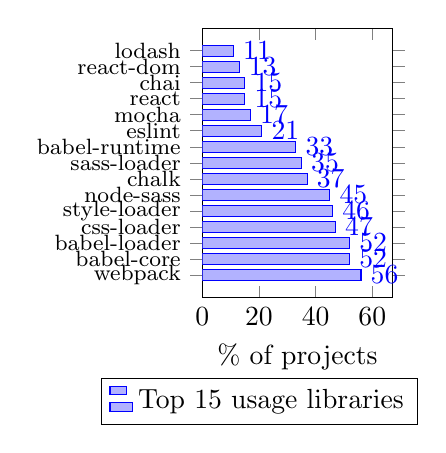
\begin{tikzpicture}
    \begin{axis}[
        xbar,
        xmin=0,
        width  = 4cm,
        height = 5cm,
        bar width=4pt,
        enlarge y limits=0.1,
        xlabel={\% of projects},
        legend style={at={(0.3,-0.30)},
      anchor=north,legend columns=-1},
        nodes near coords,
        yticklabel style={rotate=0},
        ytick = data,
        table/header=false,
        table/row sep=\\,
        yticklabels from table={\footnotesize
         {webpack}\\\footnotesize {babel-core}\\\footnotesize {babel-loader}\\\footnotesize {css-loader}\\
          \footnotesize {style-loader}\\ \footnotesize {node-sass}\\ \footnotesize {chalk}\\ \footnotesize {sass-loader}\\ \footnotesize {babel-runtime}\\ \footnotesize {eslint}\\ \footnotesize {mocha}\\ \footnotesize {react}\\ \footnotesize {chai}\\\footnotesize {react-dom}\\\footnotesize {lodash}\\
          }{[index]0},
        enlarge x limits={value=0.2,upper}
    ]
     \legend{Top 15 usage libraries}
    \addplot table[y expr=\coordindex,x index=0]{56\\52\\52\\47\\46\\45\\37\\35\\33\\21\\17\\15\\15\\13\\11\\};
  
    
    \pgfplotsinvokeforeach{0,3,4,7,8,11}{\coordinate(l#1)at(axis cs:#1,0);}
    \end{axis}
    \coordinate(bbs)at(current bounding box.south);
\end{tikzpicture}
    }}
    \subfigure[][SO npm posts]{\resizebox{0.23\textwidth}{!}{
           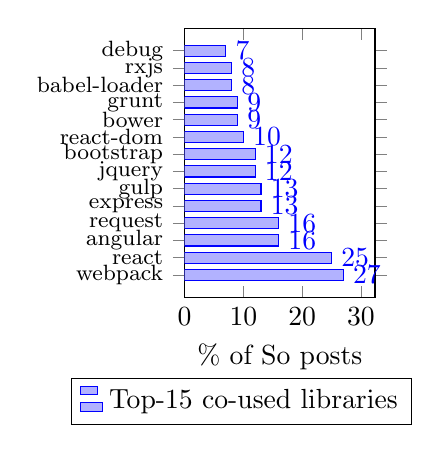
\begin{tikzpicture}
    \begin{axis}[
        xbar,
        xmin=0,
        width  = 4cm,
        height = 5cm,
        bar width=4pt,
        enlarge y limits=0.1,
        xlabel={\% of So posts},
        legend style={at={(0.3,-0.30)},
      anchor=north,legend columns=-1},
        nodes near coords,
        yticklabel style={rotate=0},
        ytick = data,
        table/header=false,
        table/row sep=\\,
        yticklabels from table={\footnotesize
         {webpack}\\\footnotesize {react}\\\footnotesize {angular}\\\footnotesize {request}\\
          \footnotesize {express}\\ \footnotesize {gulp}\\ \footnotesize {jquery}\\ \footnotesize {bootstrap}\\ \footnotesize {react-dom}\\ \footnotesize {bower}\\ \footnotesize {grunt}\\ \footnotesize {babel-loader}\\ \footnotesize {rxjs}\\\footnotesize {debug}\\\footnotesize {webpack-dev-server}\\
          }{[index]0},
        enlarge x limits={value=0.2,upper}
    ]
     \legend{Top-15 co-used libraries}
    \addplot table[y expr=\coordindex,x index=0]{27\\25\\16\\16\\13\\13\\12\\12\\10\\9\\9\\8\\8\\7\\};
  
    
    \pgfplotsinvokeforeach{0,3,4,7,8,11}{\coordinate(l#1)at(axis cs:#1,0);}
    \end{axis}
    \coordinate(bbs)at(current bounding box.south);
\end{tikzpicture}
        
    }}
    
 
    \caption{Comparison of co-used libraries between real npm projects and SO posts. Result shows that developers are likely to mention different usage libraries in SO posts compared to real projects.}
   
    \label{fig:PS1}
    \end{figure}


\begin{table*}[t]
\centering
	\caption{Comparison of inferred library usage patterns from SO posts and real npm projects. The highlghted rows represent the library usage patterns that does not exist in top 15 real npm projects usage patterns.}
	\label{tab:ps2}
% \resizebox{\textwidth}{!}{%
\begin{tabular}{@{}lc|llc@{}}
\toprule
Real npm projects libraries usage patterns & Support &  & SO posts libraries usage patterns & Support \\ \midrule
\{'babel-loader', 'webpack'\} & 0.50 &  & \{'babel-loader', 'webpack'\} & 0.07 \\
\{'babel-loader', 'babel-core'\} & 0.48 &  & \cellcolor[HTML]{999999}\{'webpack-dev-server', 'webpack'\} & 0.06 \\
\{'webpack', 'babel-core'\} & 0.47 &  & \{'css-loader', 'webpack'\} & 0.05 \\
\{'babel-loader', 'webpack', 'babel-core'\} & 0.47 &  & \cellcolor[HTML]{999999}\{'angular', 'rxjs'\} & 0.05 \\
\{'css-loader', 'webpack'\} & 0.47 &  & \cellcolor[HTML]{999999}\{'bootstrap', 'jquery'\} & 0.05 \\
\{'babel-loader', 'css-loader'\} & 0.46 &  & \cellcolor[HTML]{999999}\{'babel-loader', 'react'\} & 0.05 \\
\{'webpack', 'style-loader'\} & 0.46 &  & \cellcolor[HTML]{999999}\{'react-dom', 'webpack'\} & 0.05 \\
\{'css-loader', 'style-loader'\} & 0.46 &  & \cellcolor[HTML]{999999}\{'react', 'react-dom', 'webpack'\} & 0.05 \\
\{'babel-loader', 'css-loader', 'webpack'\} & 0.46 &  & \{'css-loader', 'style-loader'\} & 0.05 \\
\{'css-loader', 'webpack', 'style-loader'\} & 0.45 &  & \cellcolor[HTML]{999999}\{'babel-loader', 'react', 'webpack'\} & 0.04 \\
\{'babel-loader', 'style-loader'\} & 0.45 &  & \cellcolor[HTML]{999999}\{'react', 'react-scripts'\} & 0.04 \\
\{'babel-loader', 'css-loader', 'style-loader'\} & 0.45 &  & \{'webpack', 'style-loader'\} & 0.04 \\
\{'babel-loader', 'webpack', 'style-loader'\} & 0.45 &  & \{'babel-loader', 'babel-core'\} & 0.04 \\
\{'babel-loader', 'css-loader', 'webpack', 'style-loader'\} & 0.45 &  & \{'css-loader', 'webpack', 'style-loader'\} & 0.04 \\
\{'css-loader', 'babel-core'\} & 0.44 &  & \cellcolor[HTML]{999999}\{'jquery', 'webpack'\} & 0.04 \\ \bottomrule
\end{tabular}%
% }
\end{table*}


\noindent\textbf{Results. }\textbf{Developers are likely to mention different libraries in the  usage patterns of SO posts compared to real npm projects.} From Fig.~\ref{fig:PS1}(a) and (b), we observe that only 4 libraries are common from top 15 libraries between two dataset. 
In addition, we observe that although `webpack' is commonly ranked as the top most co-used library in both dataset while the rest of top co-used libraries ranks are different.

\textbf{From SO posts, we can obtain additional reusable libraries usage patterns for recommendation system.} Table~\ref{tab:ps2} shows the comparison of inferred libraries usage patterns from SO and actual usage patterns from real npm projects.  We find that the top usage patterns are different. Also, we observe that SO posts libraries usage patterns belong low support compared to real npm projects usage patterns. This indicate that, developers discuss a wide variety of usage libraries patterns in SO posts. For example, $\{`babel-loader', `webpack' \}$ is commonly ranked as the top most frequent libraries usage pattern in real npm projects with support 0.5 while in SO posts support is only 0.07.  In Table~\ref{tab:ps2}, the highlighted rows represent the SO libraries usage patterns that do not exist in the top-15 real npm projects library usage patterns.

\begin{tcolorbox}
    \textbf{Summary of RQ$_1$}: 
    Developers are likely to mention different libraries in the usage patterns of SO posts compared to real npm projects. From SO, we can infer additional reusable libraries usage patterns for recommendation system.
\end{tcolorbox}

\begin{figure}[ht]
	\centering
	\includegraphics[width=0.49\textwidth]{architecture.pdf}
	\caption{Recommendation system architecture.} 
	\label{fig:method}
\end{figure}

\section{SOLibRec: A Library Recommendation Approach}
\label{sec:SOLibRec}
The SOLibRec is a third-party library recommendation system that combines usage libraries patterns from SO posts and real projects dataset as traning resource.
It is a recommendation system that encodes relationship among usage libraries and projects by means of a semantic graph and utilize user-item collaborative filtering technique~\cite{schafer2007collaborative} to recommend third-party libraries. 
The overview of the recommendation system architecture is shown in Fig.~\ref{fig:method}. 
It consists of following software components:
\begin{itemize}
    % \item Extract usage libraries from SO posts and real projects dataset.
    \item Find the relationship among projects and usage libraries.
    \item Compute similarity to find projects, which are similar to that project under development.
    \item Recommend a set of libraries to the project using a collaborative filtering technique.
    
\end{itemize}

In the typical usage scenario of SOLibRec, we assume that a software developer is developing a new project, which is already included some libraries or the developer is evolving an existing software project.
According to Fig.~\ref{fig:method}, the developer interacts with SOLibRec system by sending a request for third-party library recommendation. 
Such kind of request contains a list of libraries that are already included in the currently developing project. 
The \texttt{Data Encoder} collects usage libraries and projects from dataset to represent them in a semantic graph. This graph is then used as a base for other components of SOLibRec.
The \texttt{Similarity calculator} computes similarity among projects to find the most similar ones to the given projects. 
The \texttt{Recommendation Engine} adopts collaborative filtering technique to select top-N similar projects. 
Finally, based on the top-N projects, SOLibRec generate a ranked list of top K-libraries and send the recommendation list to the developer.

% The background data can be collected for package-managers like npm, maven, NuGet, etc from SO posts and to support developers of different platforms.

In the following, the SOLibRec components are described in detail. 


 

\textit{\textbf{A. Data Encoder}}
A library recommendation system is based on projects and its usage libraries. In this, a project-libraries matrix is used to represent relationship between libraries and projects. A cell in the matrix is set to 1 if the library is included in the project specified by the row, it is set to 0 otherwise. For example, consider a set of projects $P=\{P1, P2, P3, P4\}$ together with a set of libraries $L=\{lib1=bcrypt; lib2=express; lib3=jade; lib4=nodeman;\}$. By observing libraries list of the four projects, we find the following inclusions: $P1\ni lib1, lib3, lib4; P2\ni lib2, lib3; P3\ni lib1, lib2, lib4; P4\ni lib2, lib4$.

\begin{figure}[ht]
\hfill
\subfigure[Matrix]{\includegraphics[width=0.20\textwidth]{matrix.pdf}}
\hfill
\subfigure[Graph ]{\includegraphics[width=0.15\textwidth, height=3.2cm]{graph_new.pdf}}
\hfill
\caption{Projects and libraries relationship}
	\label{fig:method1}
\end{figure}

\textit{\textbf{B. Similarity Calculator}}
The \texttt{Recommendation Engine} works by  relying on project-libraries matrix. To provide inputs for this module, the first task of SOLibRec is to perform similarity computation on the input projects to find the most similar projects for a given project under development. Hence, the ability to compute the similarities among projects has an effect on the recommendation outcome. We derive semantic graph representation model to show the relationships among projects and eventually calculate the similarities. Here, the semantic graph model is appropriate since it allows flexible data computation integration and computation techniques. By utilizing the graph representation, we are able to transform the set of SO posts and libraries shown in Fig.~\ref{fig:method1}(a) into directed graph as in Fig.~\ref{fig:method1}(b). 
% We adopted our proposed SOLibRec approach~\cite{nguyen2020crossrec} to compute the similarity among projects graph nodes. 
In the graph, two nodes are deemed to be similar if they point to the same node with same edge. For example, by observing the graph in Fig.~\ref{fig:method1}(b), we can notice that $P_1$ and $P_3$ are higly similar since they both point to the same two nodes $lib_1, lib_4$. 

Using this metric, the similarity between two project nodes $P$ and $q$ in the graph is computed by considering their feature sets~\cite{di2012linked}. Let us assume that $P$ has a set of neighbour nodes $( lib_1, lib_2, ...lib_i)$, the features of $P$ is represented by a vector $\vv{\phi_{p}}= \{ \phi_1, \phi_2, ..\phi_{pi}\}$ where $\phi_{pi}$ is the weight of node $lib_i$. It is computed as the term-frequency and inverse document frequency value as follows: 
% \begin{align}
%     \begin{split}\label{eq:1}
%     O_i ={}& TF-IDF\ Score\\
%         {}& = TF_{lib_i}\times IDF \\
%         {}& = TF_{lib_i}\times \log\frac{|P|}{df_{lib_i}}\\
% \end{split}
% \end{align}

\begin{eqnarray}
    O_i & = & TF_{lib_i}\times \log\frac{|P|}{df_{lib_i}}
\end{eqnarray}


Where $TF_{lib_i}$ is the frequency of $lib_i$ with respect to $P$, it can be eighter 0 and 1 since there are maximum one $lib_i$ connected to $P$ by the edge includes; $|P|$ is the total number of projects considered; $df_{lib_i}$ is the number of projects connecting to $lib_i$ via the edge includes. Thus, the similarity between two projects $P$ and $q$ with their corresponding feature vectors $\vv{\phi_p}= \{ \phi_1, \phi_2, ..\phi_{pi}\}$ and $\vv{\omega_{q}}= \{ \omega_1, \omega_2, ..\omega_{qi}\}$ is computed as given below:

\begin{eqnarray}
    Similarity (p,q) & = & \frac{\sum_{i=1}^{n} \phi_{pi}.\omega_{qi}}{\sqrt{\sum_{i=1}^{n} \phi_{pi}^2} \sqrt{\sum_{i=1}^{n} \omega_{qi}^2}}
\end{eqnarray}


Where n in the cardinality of the set of libraries that $p$ and $q$ share in common. Intuitively, $p$ and $q$ are characterized by using vectors in an n-dimensional space and measure the cosine of the angle between two vectors.


\textit{\textbf{C. Recommendation Engine.}}
 In the context of SOLibRec, we utilize user-item collaborative filtering technique as a engine to recommend libraries. Given a project under development $P$, the inclusion of currently used libraries in $P$ can be deduced from projects that are similar to $P$. The process is summarized as follows:
\begin{itemize}
    \item Compute similarities between project under development and all the projects in the collection;
    \item select top-N most similar projects; and
    \item predict libraries by means of those collected projects.
\end{itemize}

Our next step is to compute a recommendation score for each library obtained from top-N similar projects. We compute the score of each library using same approach utilized by previous study~\cite{di2015recommender}. Given a library $lib_i$, we compute the collaborative filtering based recommendation score for $lib_i$ to predict if $P$ should include it as follows:

\begin{eqnarray}
    r_{p,lib_{i}} & = & \overline{r_{p}}+ \frac{\sum_{q\epsilon topsim(p)} (r_{q, lib_{i}}-\overline{r_{q}}).sim(p,q)}{\sum_{q\epsilon topsim(p)} r_{q, lib_{i}}.sim(p,q)}
\end{eqnarray}

In the above equation, $\overline{r_{p}}$ and $\overline{r_{q}}$ are the mean of the rating of $p$ and $q$, respectively. the project $q$ belongs to top-N similar projects, denoted as $topsim(p)$, $sim(p,q)$ is the similarity score between two projects $p$ and $q$.
 

% \subsection{SOLibRec in action}

\section{Empirical Evaluation}
\label{sec:evaluation}
We perform an empirical study to evaluate the effectiveness of SOLibRec. First, we describe the goal and research questions we addressed. Second, we describe the studied systems that we used to evaluate. Third, we present evaluation metrics. Lastly, we describe our baseline comparison approach.
\\

\noindent\textbf{A. Goal and Research Questions}\\

The goal of our empirical study is to evaluate the effectiveness of SOLibRec in term of accuracy in recommending third-party libraries to other systems. The results of SOLibRec are then compared with CrossRec~\cite{nguyen2020crossrec} as a baseline approach.
\begin{itemize}
        
        \item{\RqTwo}
        We propose SOLibRec to find appropriate third-party library to software under development based on project-libraries similarity. We aim to evaluate the performance of our approach in term of precision and recall. Better performing approaches are of great value to practitioners since they allow them to take better informed decisions. 
         
        \item{\RqThree}
        Recommending correct third-party libraries could ease developers as well as avoid interfering unrelated libraries. We are interested in understanding the rationale behind the performance difference between two system.
        
        % The higher ranks of the correct libraries that the approach can recommend, the more effective it is. We set out this research question to evaluate the overall performance of our approach in the view of ranking for a recommendation.
        % We suppose that SOLibRec with more data as query enhance the overall performance. The hypothesis is increase of dataset size using SO npm library usage dataset will help to improve its performance.
    \end{itemize}

\noindent\textbf{B. Studied Dataset}\\

To evaluate SOLibRec, we use two dataset obtained in section~\ref{sec:prelimanary}, i.e., SO and libraries.io npm usage libraries dataset. Fig.~\ref{fig:distribution} shows the distribution of co-used libraries for real npm projects and SO npm posts.
In the dataset preparation step we have two types of data namely training and testing set. The SOLibRec utlize the SO and libraries.io npm usage libraries dataset for training, while the CrossRec only utilize the libraries.io npm usage libraries dataset for training. Finally for testing performance of both system, we utilize same sample projects libraries usage dataset from libraries.io which does not exist in the training set. Table~\ref{tab:summary} illustrates the summary of used dataset by the recommendation systems.\\

\begin{table}[]
\caption{Summary of the dataset source used for each recommendation system}
\label{tab:summary}
\resizebox{0.49\textwidth}{!}{%
\begin{tabular}{@{}llll@{}}
\toprule
\begin{tabular}[c]{@{}l@{}}Recommender\\ system\end{tabular} & \begin{tabular}[c]{@{}l@{}}Training  \\ dataset\end{tabular} & \begin{tabular}[c]{@{}l@{}}Testing\\ dataset\end{tabular} & \begin{tabular}[c]{@{}l@{}}\# project \\ rows\end{tabular} \\ \midrule
CrossRec & libraries.io (80\%) & libraries.io (20\%) & 9438 \\
SOLibRec & SO (100\%)+libraries.io (80\%) & libraries.io (20\%) & 8012+9438 \\ \bottomrule
\end{tabular}%
}
\end{table}

\begin{figure}[t]
    \centering
    {\resizebox{0.30\textwidth}{!}{
        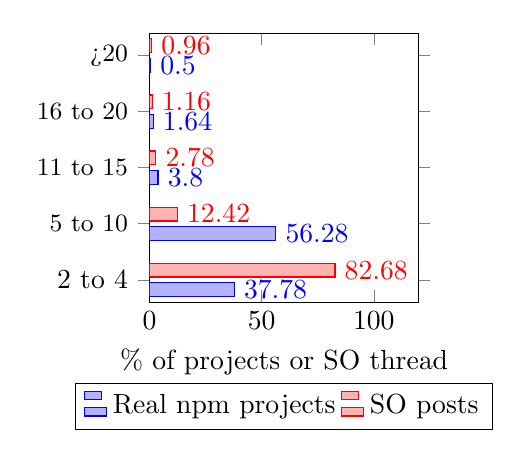
\begin{tikzpicture}
    \begin{axis}[
        xbar,
        xmin=0,
        xmax=100,
        width  = 5cm,
        height = 5cm,
        bar width=5pt,
        enlarge y limits=0.1,
        xlabel={\% of projects or SO thread},
           legend style={at={(0.5,-0.3)},
      anchor=north,legend columns=-1},
        nodes near coords,
        % yticklabel style={rotate=45},
        ytick = data,
        table/header=false,
        table/row sep=\\,
        yticklabels from table={\normalsize
         {2 to 4}\\\small {5 to 10}\\\small {11 to 15}\\\small {16 to 20}\\
          \small {>20}\\
          }{[index]0},
        enlarge x limits={value=0.2,upper}
    ]
     \legend{Real npm projects, SO posts}
    \addplot table[y expr=\coordindex,x index=0]{37.78\\56.28\\3.80\\1.64\\0.50\\};
    \addplot table[y expr=\coordindex,x index=0]{82.68\\12.42\\2.78\\1.16\\0.96\\};
 
    \pgfplotsinvokeforeach{0,3,4,7,8,11}{\coordinate(l#1)at(axis cs:#1,0);}
    \end{axis}
    \coordinate(bbs)at(current bounding box.south);
\end{tikzpicture}
    }}
  
 
    \caption{Distribution of co-used libraries between real npm projects and SO posts dataset.}
   
    \label{fig:distribution}
    \end{figure}


 

\noindent\textbf{C. Evaluation Metrics}\\

To compare the performance of SOLibRec, there are several metric available to evaluate the ranked list of recommended items. Accuracy is considered as one of the most important quality indicator for information retrieval system~\cite{saracevic1995evaluation}. In our case, we are interested to calculate accuracy in term of precision and recall for top k recommended libraries. Precision@k is the ratio of the top-K recommended libraries that belong to ground-truth dataset, whereas the recall@k is the ratio of ground truth libraries that appear in the k recommended items. We use the following formula~\cite{herlocker2004evaluating} for calculating the precision and recall:

\begin{eqnarray}
    Precision@ k & = & \frac{|match_{k}(P)|}{K}
\end{eqnarray}
\begin{eqnarray}
    Recall@k & = & \frac{|match_{k}(P)|}{|GT(P)|}
\end{eqnarray}

where, $|match_{k}(P)|$= \# of recommended relevant libraries, $K$= \# of recommended libraries, and $|GT(P)|$= \# of relevant ground-truth libraries.
In the context of SOLibRec we are most likely interested in recommending top-k libraries from top-N nearest neighbour projects. Here, we will tune the parameters (K and N) of SOLibRec to check the library recommendation performance. Finally, we compute the relative improvement (RI) to highlight the SOLibRec performance\footnote{RI:\url{https://tinyurl.com/yyo8jq6k}}. \\

% So it makes more sense to compute precision and recall metrics in the first k items instead of all the items. Thus the notion of precision and recall at k where k is the number of libraries exploited for recommendation process from N-nearest neighbour projects. 

\noindent\textbf{D. CrossRec: A Baseline Approach}\\

We re-implement the CrossRec~\cite{nguyen2020crossrec} as our baseline. CrossRec is a system for providing third-party library recommendations. It encodes relationships among various OSS artifacts by means of semantic graph and utilize user-item collaborative filtering to recommend third-party libraries to the project under development. The calculation of CrossRec can be summarized as follows, (1) represent relationships among projects and libraries retrieved from existing repositories; (2) compute similarities to find among training projects and projects under development; (3) recommend libraries to projects using user-item collaborative filtering technique.To conserve space, a full description of the CrossRec is provided in~\cite{nguyen2020crossrec}.


\section{Results} 
\label{sec:results}
In this section, we report and discuss the results of empirical evaluation with respect to our research questions. For each research questions, we present its approach and results.\\

\noindent\textit{\RqTwo}\\

\noindent\textbf{Approach.} To address RQ$_2$, we execute SOLibRec for every projects in chronological order to obtain the lists for recommended libraries. To evaluate how accurately the SOLibRec can correctly recommended libraries, we compute the top-k libraries from top-N most similar projects. We also compute the results of our approach with CrossRec.\\

% Since SOLibRec leverage the SO and libraries.io projects usage libraries dataset  to recommend libraries, we perform an experiment based on realistic scenario.

\begin{table}[]
\caption{Performance comparison of SOLibRec and CrossRec}
\label{tab:results}
\resizebox{0.48\textwidth}{!}{%
\begin{tabular}{@{}l|cc|cc|cc@{}}
\toprule
Params & \multicolumn{2}{c|}{SOLibRec} & \multicolumn{2}{c|}{CrossRec} & \multicolumn{2}{c}{Relative improvement} \\ \midrule
N, k & Precision & Recall & Precision & Recall & Precision (\%) & Recall (\%) \\ \midrule
2, 5 & 0.02  & 0.07 & 0.02 & 0.06 & 0.00 & \textbf{16.67} \\
5, 5 & 0.04 & 0.12 & 0.03 & 0.11 & \textbf{33.33} & \textbf{9.00} \\
5, 10 & 0.03 & 0.14 & 0.03  & 0.15 & 0.00  & -6.67 \\
10, 10 & 0.03 & 0.20 & 0.03 & 0.21 & 0.00 & -4.76 \\
10, 15 & 0.03 & 0.22 & 0.03 & 0.23 & 0.00 & -4.35 \\
10, 20 & 0.03 & 0.23 & 0.03 & 0.24 & 0.00 & -4.17 \\ \bottomrule
\end{tabular}%
}
\end{table}

\noindent\textbf{Result.} \textbf{SOLibRec shows 33.33\% relative improvement in precision compared to CrossRec for N=5 and k=5 parameter settings.} Table~\ref{tab:results} shows the comparison of performance between SOLibRec and CrossRec. We observe that the rest of parameter setting couldn't achieve relative improvement in precision. This indicates that SOLibRec is better from practitioners perspective.

Again, \textbf{the SOLibRec shows 9.00 to 16.67\% relative improvement in recall compared to CrossRec for K=5 and N=2, 5 parameter settings.} From Table~\ref{tab:results} we observe that as the number of recommended libraries increases, the recall score of SoLibRec also decreases. The reason for decreasing the recall of SOLibRec is the distirbution of SO Posts usage libraries dataset illustrated in Fig.~\ref{fig:distribution}. We observed that 82.68\% libraries usage patterns from SO posts consists of only 2-4 libraries. Hence, it reduce the chance to obtain top similar projects with higher number of libraries.

\begin{tcolorbox}
    \textbf{Summary of RQ$_2$}: 
    SOLibRec shows 33.33\% relative improvement in precision compared to CrossRec for N=5 and k=5 parameter settings. Again, the SOLibRec shows 9.00 to 16.67\% relative improvement in recall compared to CrossRec for K=5 and N=2, 5 parameter settings.
\end{tcolorbox}


\noindent\textit{\RqThree}\\

\noindent\textbf{Approach.} To address RQ$_3$, we carefully analyze the internal architecture of two recommendation system to understand the reason of performance difference. \\

\noindent\textbf{Result.} \textbf{SOLibRec outperforms the baseline approach due to the additional training resources from SO posts although their internal recommendation architectures are same.} In detail, the SOLibRec uses the additional training data resource from SO posts, while CrossRec uses only the training resource from libraries.io projects. Therefore the performance of CrossRec is limited due to lack of training resources.\\

\begin{tcolorbox}
    \textbf{Summary of RQ$_3$}: 
    SOLibRec outperforms the baseline approach, CrossRec due to additional training resource (i.e., SO posts).
\end{tcolorbox}

\section{Discussion}
\label{sec:discussion}
In this section, we discuss the applicability of SOLibRec. We also discuss the threats to validity of our study.\\

% \noindent\textit{Performance: Why does SOLibRec outperform CrossRec?}\\
% The resuts of our empirical study evaluation shows that the proposed approach, SOLibRec outperforms the baseline approach, CrossRec. The difference between SOLibRec and CrossRec is due to the additional libraries usage dataset from SO posts although their internal recommendation architecture are same. In detail, the SOLibRec uses the additional training data resource from SO posts, while CrossRec uses only the training resource from libraries.io projects.Therefore the performance of CrossRec is limited due to lack of training resources.\\

\noindent\textit{Applicability: Can SOLibRec effectively help developers find appropriate libraries?}\\
In RQ$_1$, the results of our exploratory study show that SO posts discuss a wide variation of usage libraries patterns and thereby useful as addition training resource of recommendation system. To confirm how effectively SOLibRec help developers, we execute SOLibRec to recommend libraries. We found that, SOLibRec can achieve 33.33\% relative improvement in precision which is very favourable from practitioners perspective. Again, SOLibRec can achieve up to 16.67\% relative improvement in recall which is also reasonable from researchers perspective. Thus, we believe that SOLibRec can help developers find appropriate libraries and speed up the overall software development process.\\

\noindent\textbf{Threat to validity.} We discuss potential threats to validity of our work as follows:

\textit{Internal Validity. }  Threats to internal validity refers to experimental bias. Most of our experimental process is automated and randomized. Thus we believe that there is little experimental bias.

\textit{External validity. } Threats to external validity refers to generalizability of our findings. Our datasets consists of npm projects usage libraries from libraries.io and SO posts. SO is a popular platform for question and answers from developers with a wide variety of domains and experts. Hence, our observations and results can not be generalized for other types of package managers like julia. In addition, we consider only top 100 npm libraries. Selecting more libraries may cause variation of SOLibRec results. 

\textit{Construct validity. } Threats to construct validity refers to the suitability of our evaluation measure. Currently, we use precision@k and recall@k to measure the effectiveness of our approach. This is well measurement approach that is also used in previous studies~\cite{thung2013automated, nguyen2020crossrec}.

\section{Conclusion And Future Work}
\label{sec:conclusion}
In this paper,we empirically investigate the SO posts libraries usage patterns. From our quantitative examination, we find that, SO posts can be useful resource to obtain additional libraries usage patterns. 

To help developers find appropriate libraries, we propose SOLibRec, a recommendation system that combines usage libraries patterns from SO posts and real projects dataset. In order to evaluate SOLibRec, we perform a case study on npm projects usage libraries from SO posts (8012) and libraries.io (9438) dataset. Our empirical evaluation shows that, SOLibRec outperform the baseline approach with 33.33\% relative improvement in precision and 9.00 to 16.67\% in Recall at top 5 recommended libraries. Therefore, we believe that SOLibRec can help developers find appropriate libraries and speed the overall software development process.

In our future work, we will deploy SOLibRec in a development environment and perform experiments with developers to analyze how effectively and practically SOLibRec can help developers in recommending third-party libraries.

% \subsection{Research questions}
% Our empirical study is divided into two research question. Here we will discuss the SOLibRec performance for the two dataset D1 and D2.
    
%     \begin{itemize}
%         \item{\RqOne} We evaluate the SOLibRec by considering SO usage third-party library and real npm projects.  
%         \item{\RqTwo} Apart from success rate, we investigate if the approach good performance in term of accuracy and novelty.
%         \item{\RqThree} We suppose that SOLibRec with more data as query enhance the overall performance.
%     \end{itemize}
    
 
% \section{Library recommendation system proposal}




\bibliographystyle{ieicetr}
\bibliography{reference}
%\bibliographystyle{ieicetr}% bib style
%\bibliography{}% your bib database
% \begin{thebibliography}{99}% more than 9 --> 

% \bibitem{}
% \end{thebibliography}

%\profile{}{}
%\profile*{}{}% without picture of author's face

% \balance

\end{document}
